
\section{Formal definition of \lsystem}

\lsystem $L$ is formally a triplet $L = (\Sigma, \omega, R)$, where

\begin{itemize*}
	\item $\Sigma$ is an \emph{alphabet}, a non-empty set of symbols, $\Sigma^{*}$ is a set of all the words\footnote{A word is a sequence of symbols.} which can be created from the alphabet $\Sigma$, $\Sigma^{+}$ is a set of all non-empty words which can be created from the alphabet $\Sigma$,
	\item $\omega \in \Sigma^{+}$ is an \emph{axiom} (also called seed), a word defining the initial state of the \lsystem,
	\item $R \subset \Sigma \times \Sigma^{*}$ is a finite set of \emph{rewrite rules} (production rules), a rewrite rule defines rewriting of a symbol $s \in \Sigma$ to a word $w \in \Sigma^{*}$ is written as $s \rightarrow w$.
\end{itemize*}

For any symbol $s \in \Sigma$ which does not appear on the left-hand side of any rewrite rule in $R$, the identity rewrite rule $s \rightarrow s$ is assumed.
These symbols are called constants or terminals.

The formal definition of an \lsystem is similar to a deterministic context-free grammar but there are a few differences.
In such a grammar we distinguish between terminal and non-terminal symbols, but in \lsystems we do not define them explicitly (rather we define the identity rewrite rule for terminal symbols in \lsystems).
The next difference is in the initial string.
In the grammar there is only one symbol as an initial state but the \lsystem allows a non-empty word.
The biggest difference, however, is in the rewriting principles which are described in the following section.


\subsection{Rewriting principles of an \lsystem}

Starting with the initial axiom (0th iteration), in each iteration \emph{all} symbols are rewritten with rewrite rules to form next iteration.
All symbols can be rewritten because every symbol is on the left side of some rewrite rule.
% (if symbol have not been on the left side of some rewrite rule, identity rule would be defined).
There is only one way to rewrite symbols in an iteration, thus rewriting is deterministic.
The result depends only on the axiom.

The rewriting of symbols is parallel (all symbols are rewritten simultaneously during each iteration).
This means that when some symbols are rewritten, the resulting symbols are not rewritten again in the same iteration.

The described rewriting principles distinguish an \lsystem from a formal grammar.
In the grammar it is not mandatory to rewrite all possible symbols (the derivation of start state can result in several different derivations).
Thus, \lsystems are a strict subset of languages.

The \lsystem in \autoref{lsys:rrExample} produces strings as shown in \autoref{fig:rrExampleResult}.
The \lsystem starts with an axiom \texttt{A} and two rewrite rules \texttt{A} $\rightarrow$ \texttt{B} and \texttt{B} $\rightarrow$ \texttt{A}, \texttt{B}.
In the first iteration the axiom \texttt{A} is rewritten by the first rewrite rule to \texttt{B}.
In the second iteration \texttt{B} is rewritten with the second rewrite rule to symbols \texttt{A}, \texttt{B}.
In the third iteration the first symbol \texttt{A} is rewritten to \texttt{B} and the second symbol \texttt{B} rewritten to \texttt{A}, \texttt{B} which gives string \texttt{B}, \texttt{A}, \texttt{B} and so on.

\begin{Lsystem}[label=lsys:rrExample,caption={A simple \lsystem as an example of rewriting principles}]
lsystem RewritingExample {
	set symbols axiom = A;
	set iterations = 6;
	set interpretEveryIteration = true;
	@rewrite A to B;@
	@rewrite B to A B;@
}
process all with SymbolPrinter;
\end{Lsystem}

\begin{table}[h]
	\centering
	\begin{tabular}{c l}
   		\toprule
   		Iteration & String of symbols \\
   		\midrule
		0 & A \\
		1 & B \\
		2 & A B \\
		3 & B A B \\
		4 & A B B A B \\
		5 & B A B A B B A B \\
		6 & A B B A B B A B A B B A B \\
		\bottomrule
	\end{tabular}
	\caption{Result of the \lsystem in \autoref{lsys:rrExample}}
	\label{fig:rrExampleResult}
\end{table}


\subsection{Interpretation of \lsystem symbols}

The result of an \lsystem rewriting is a string of symbols.
As mentioned in the \nameref{sec:Introduction}, we can interpret a string of symbols in many ways: for example, as computer graphics or music.

The simplest and most common interpretation of \lsystem symbols is to interpret them as 2D graphic elements like lines or polygons.
This interpretation is often called \emph{turtle graphics} and it will be used to interpret most of the \lsystems in this thesis.
This approach can be easily extended into 3D.

Let symbol \texttt{F} be interpreted as \emph{draw line forward}, \texttt{+} as \emph{turn left} and \texttt{-} as turn right.
\autoref{fig:intSequences} shows the strings of symbols interpreted using turtle graphics.
The initial direction is to the right.

\begin{figure}[h]
	\centering
	\subfloat[$F + F - - F + F$, turning angle: $60^{\circ}$]{
		
\includegraphics[scale=1]{IntTriangle}
	} ~
	\subfloat[$F + F - F - F + F$, turning angle: $90^{\circ}$]{
		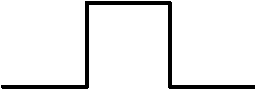
\includegraphics[scale=1]{IntSquare}
	} ~
	\subfloat[$F + F + + F - F - - F F - F$, turning angle: $60^{\circ}$]{
		\hspace{9mm}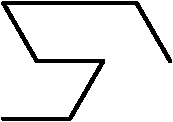
\includegraphics[scale=1]{IntHexa}\hspace{9mm}
	}
	\caption{Examples of interpretation of simple string of symbols}
	\label{fig:intSequences}
\end{figure}


A slightly more complex string of symbols, as an example of interpretation, is generated by the \lsystem in \autoref{lsys:intExampleCode}, where symbol \texttt{F} is interpreted as \emph{draw line forward},
	symbol \texttt{+} is interpreted as \emph{turn left} by 85 degrees and symbol \texttt{-} as \emph{turn right} by 85 degrees (equally as \emph{turn left} by $-85$ degrees).
The result of interpretation of the first, second and fourth iteration is in shown \autoref{fig:intExample}.

\begin{Lsystem}[label=lsys:intExampleCode,caption={Another symbol interpretation example}]
lsystem InterpretationExample {
	set symbols axiom = F;
	set iterations = 4;
	@interpret F as DrawForward(10);@
	@interpret + as TurnLeft(85);@
	@interpret - as TurnLeft(-85);@
	rewrite F to F + F - - F + F;
}
process all with SvgRenderer;
\end{Lsystem}

\begin{figure}[h]
	\subfloat{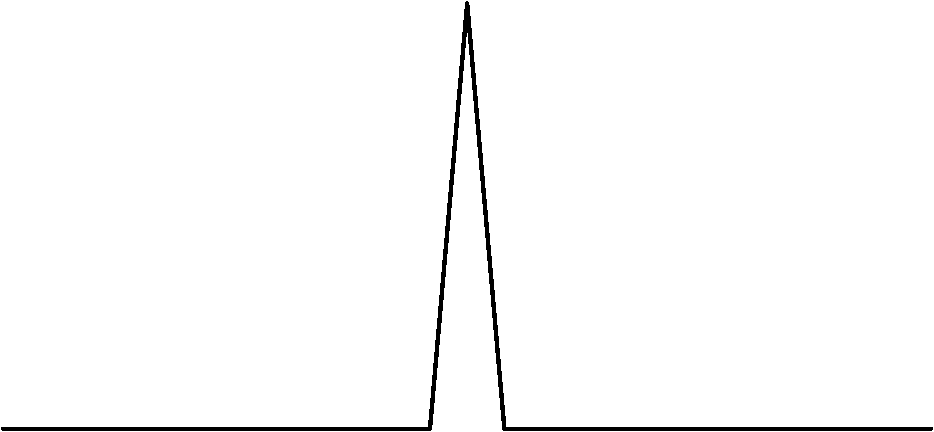
\includegraphics[scale=0.5]{Interpretation1}} \hfill
	\subfloat{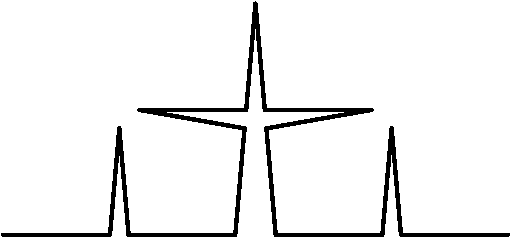
\includegraphics[scale=0.5]{Interpretation2}} \hfill
	\subfloat{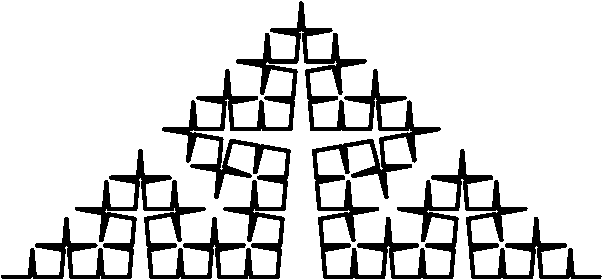
\includegraphics[scale=0.5]{Interpretation4}}
	\caption[The first, second and fourth iteration of the Cesaro curve]{The first, second and fourth iteration of the Cesaro curve (\autoref{lsys:intExampleCode})}
	\label{fig:intExample}
\end{figure}

\begin{figure}[h]
	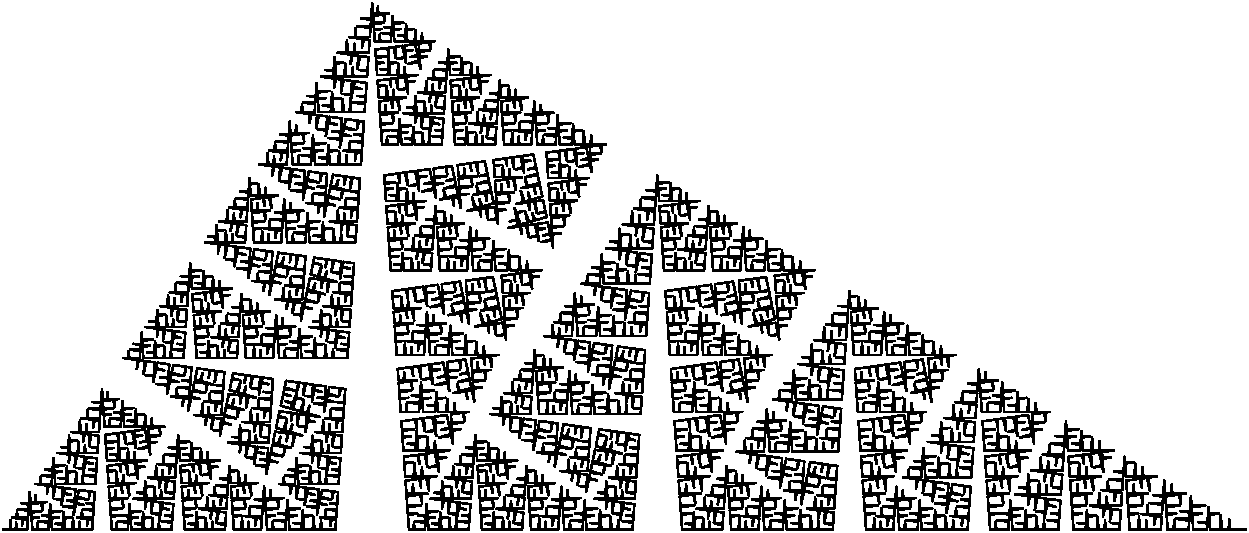
\includegraphics[width=1\linewidth]{RowOfTrees}
	\caption[Enhanced Cesaro curve]{Enhanced Cesaro curve from \autoref{fig:intExample} \cite[p.~48]{PL91}}
	\label{fig:rowOfTrees}
\end{figure}


































